\documentclass[twocolumn, a4paper, polish, 10pt]{article}
\usepackage[polish]{babel}
\usepackage[T1]{fontenc}
\usepackage{secdot}
\usepackage{indentfirst}
\usepackage{graphicx}
\usepackage{titlesec}
\usepackage[dvipsnames,svgnames,table]{xcolor}
\definecolor{fiolet}{cmyk}{0.47,1,0.07,0.33}
\usepackage[a4paper, hmargin=2cm, tmargin=1.5cm, bmargin=3cm, footskip=2cm]{geometry}
\usepackage{fancyhdr}

% Additional imports
\usepackage{xurl}
\usepackage{hyperref}
\usepackage{amsmath}
\usepackage{amssymb}
\usepackage{physics}
\usepackage{microtype}
\usepackage[colorinlistoftodos]{todonotes}
\usepackage{tikz}
\usepackage{pgfplots}
\usepackage{csquotes}

\hypersetup{
    colorlinks=true,
    linkcolor=black,
    urlcolor=blue,
    citecolor=blue
}
\setlength {\marginparwidth }{2cm}
\pgfplotsset{compat=1.18}

\pagestyle{fancy}
\lhead{}
\chead{}
\rhead{}
\cfoot{}
\rfoot{\emph{Paweł~Konopka}}
\renewcommand{\headrulewidth}{0pt}
\renewcommand{\thefootnote}{\fnsymbol{footnote}}
\cfoot{\thepage{}}

\newcommand{\RC}{\ensuremath{ R_{\mathrm{C}} }}
\newcommand{\RNi}{\ensuremath{ R_{\mathrm{Ni}} }}
\newcommand{\RPi}{\ensuremath{ R_{\mathrm{Pt}} }}

\newcommand{\RO}{\ensuremath{ R_{\mathrm{O}} }}
\newcommand{\RM}{\ensuremath{ R_{\mathrm{M}} }}

\newcommand{\ROT}{\ensuremath{ R_{\mathrm{O, T}} }}
\newcommand{\RMT}{\ensuremath{ R_{\mathrm{M, T}} }}

\newcommand{\kOhm}{\ensuremath{ \mathrm{k\Omega} }}

\begin{document}

\titleformat*{\section}{\large\bfseries\centering}
\titleformat*{\subsection}{\normalsize\bfseries}
\titleformat*{\subsubsection}{\small\bfseries}

\twocolumn[
\begin{@twocolumnfalse}
\begin{center}
\textbf{\large{Temperaturowa zależność oporu przewodników}}
\bigskip
\\Paweł~Konopka\footnotemark \\ \small{opiekun: dr Paweł Nita}\\\textit{I Pracownia Fizyczna,
Instytut Fizyki UJ}\\
\small{data rozpoczęcia ćwiczenia: 25 marca 2026}\\
\end{center}

%Abstrakt
\begin{quote}\small{
\begin{quote}
\begin{center}
\textbf{Streszczenie}
\end{center}
Celem ćwiczenia było zbadanie temperaturowej zależności oporu oraz wyznaczenie temperaturowego współczynnika oporu właściwego $\alpha$ dla oporników wykonanych z różnych przewodników. Pomiary przeprowadzono z wykorzystaniem metody równoważenia mostka Wheatstone'a. W temperaturze pokojowej zweryfikowano również teoretyczne przewidywania dotyczące oporu zastępczego dla połączeń szeregowych i równoległych. Pomiary układów oporników w większości potwierdziły założenia teoretyczne. Wyznaczenie współczynnika $\alpha$ dla opornika węglowego zakończyło się niepowodzeniem ze względu na zbyt małą dokładność aparatury w stosunku do mierzonych zmian oporu. Z kolei dla opornika niklowego uzyskano zadowalający wynik $\alpha_{\mathrm{Ni}} = 5.52(37) \cdot 10^{-3}~\frac{1}{ \mathrm{K} }$, który jest bliski wartości tablicowej.
\end{quote}
}
\end{quote}
 \bigskip
    \bigskip
\end{@twocolumnfalse}
]
\footnotetext{pawel.konopka@student.uj.edu.pl}

\section{Podstawy teoretyczne}
\subsection{Łączenie oporników szeregowo}
Jeśli $n$ oporników o oporach $(R_1, R_2, \dots, R_n)$ połączymy szeregowo, to otrzymany układ będzie miał opór zastępczy $R$ opisany równaniem~(\ref{eq:oporniki-szeregowo-teoria})~\cite{pracownia-fizyczna-e3}.
\begin{equation}
    R = \sum_{i=0}^n R_i
    \label{eq:oporniki-szeregowo-teoria}
\end{equation}

\subsection{Łączenie oporników równolegle}
Jeśli $n$ oporników o oporach $(R_1, R_2, \dots, R_n)$ połączymy równolegle, to otrzymany układ będzie miał opór zastępczy $R$ opisany równaniem~(\ref{eq:oporniki-rownolegle-teoria})~\cite{pracownia-fizyczna-e3}.
\begin{equation}
    \frac{1}{R} = \sum_{i=0}^n \frac{1}{R_i}
    \label{eq:oporniki-rownolegle-teoria}
\end{equation}

\subsection{Zależność oporu przewodnika od temperatury}
Zależność oporu przewodnika $R$ od temperatury $T$ opisana jest wzorem~(\ref{eq:teoria:temperaturowy-wspolczynnik-opornosci}), gdzie:
\begin{itemize}
    \item $T_0$ - temperatura odniesienia ($T_0 = 20^{\circ}\mathrm{C}$)
    \item $R_0$ - opór przewodnika w temperaturze $T_0$
    \item $\alpha$ - temperaturowy współczynnik oporności właściwej (stała materiałowa)
\end{itemize}

\begin{equation}
    \alpha = \frac{ R_{\mathrm{T}} - R_0 }{ R_0 \left( T - T_0 \right) }
    \label{eq:teoria:temperaturowy-wspolczynnik-opornosci}
\end{equation}

Równanie~(\ref{eq:teoria:temperaturowy-wspolczynnik-opornosci}) jesteśmy w stanie przekształcić do postaci wzoru~(\ref{eq:teoria:opor-od-temperatury}).
\begin{equation}
    R = \alpha R_0~T + \left(1 - \alpha T_0 \right) R_0
    \label{eq:teoria:opor-od-temperatury}
\end{equation}

Poprzez dopasowanie prostej $y=ax+b$ dla pomiarów oporu w danej temperaturze: ${(x, y) = (T, R)}$, a więc $R = aT + b$, jesteśmy w stanie użyć wzoru~(\ref{eq:teoria:opor-od-temperatury}), aby powiązać nieznane $\alpha$, $R_0$ z otrzymanymi $a$, $b$ oraz stałym $T_0$, co przedstawiają zależności~(\ref{eq:teoria:wspolczynniki-dopasowanej-prostej}).
\begin{equation}
\begin{split}
    a &= \alpha R_0 \\
    b &= \left(1 - \alpha T_0 \right) R_0
    \label{eq:teoria:wspolczynniki-dopasowanej-prostej}
\end{split}
\end{equation}

Zależności~(\ref{eq:teoria:wspolczynniki-dopasowanej-prostej}) można użyć, aby wyznaczyć wzór~(\ref{eq:teoria:alpha-od-prostej}) na temperaturowy współczynnik oporności właściwej $\alpha$ od uzyskanych współczynników prostej $a$ i $b$ oraz stałej $T_0 = 20^{\circ}\mathrm{C}$.
\begin{equation}
    \alpha = \left( \frac{b}{a} + T_0 \right)^{-1}
    \label{eq:teoria:alpha-od-prostej}
\end{equation}

\subsection{Mostek Wheatstone'a}
Mostek Wheatstone'a to układ pomiarowy pozwalający na precyzyjne wyznaczenie nieznanego oporu elektrycznego bez konieczności bezpośredniego pomiaru napięcia i natężenia prądu. Składa się on z czterech oporników połączonych w czworobok, czułego galwanometru (mikroamperomierza) oraz źródła zasilania napięciem stałym, które są włączone w przekątne tego układu. Pomiary polegają na doprowadzeniu mostka do stanu zrównoważonego, w którym potencjały odpowiednich węzłów są równe, a przez galwanometr nie płynie prąd ($U_{CD}=0$). W przypadku, gdy dwa znane oporniki w układzie mają taką samą wartość rezystancji, opór badanego elementu jest równy oporowi nastawionemu na opornicy dekadowej w momencie zrównoważenia układu~\cite{pracownia-fizyczna-e3}. Rysunek~\ref{fig:schemat-e3} przedstawia schemat mostka Wheatstone'a.

\begin{figure}[ht]
  \centering
  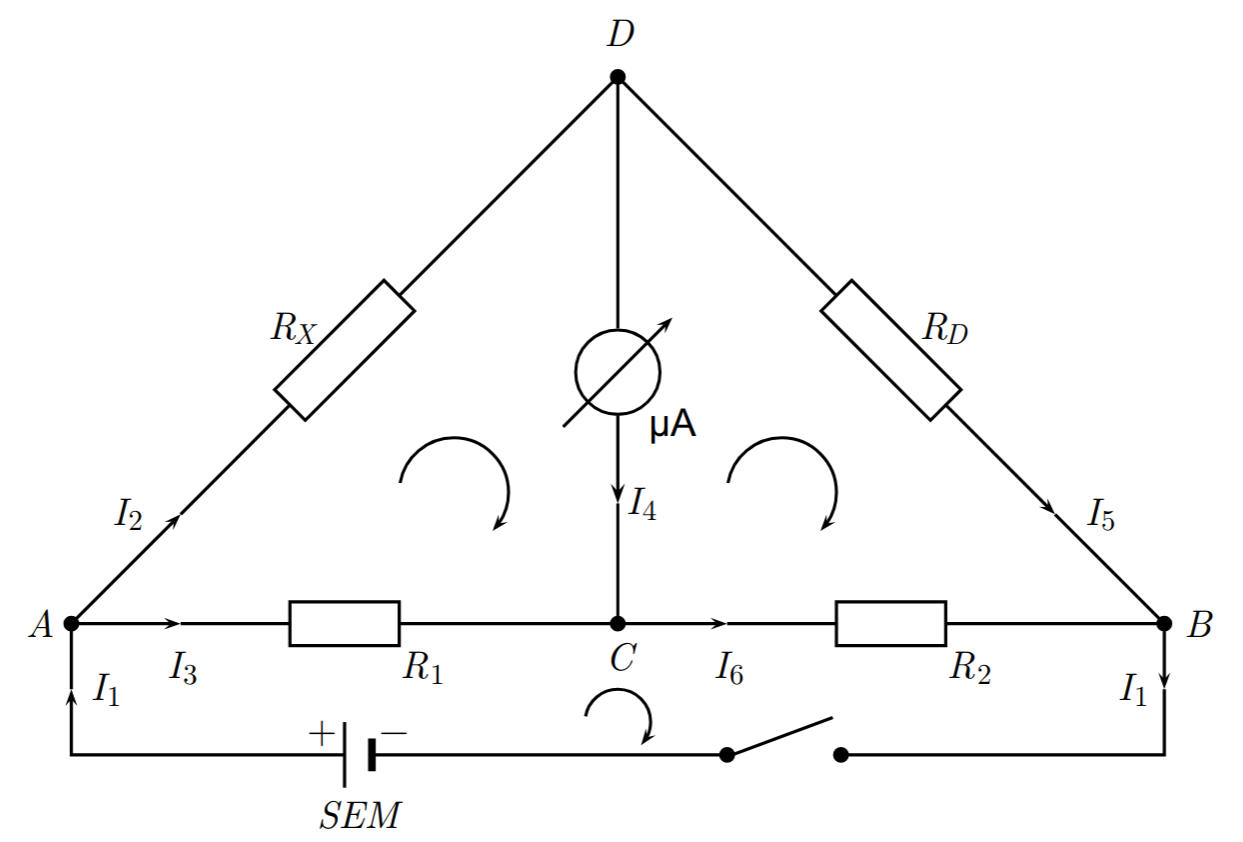
\includegraphics [width=0.95\columnwidth] {img/e3-schemat.png}
  \caption{\small
  Schemat układu doświadczalnego przedstawiający mostek Wheastone'a.
  Źródło: I~Pracownia Fizyczna, \emph{Badanie ruchu obrotowego bryły sztywnej (M7)}, Instytut Fizyki~UJ~\cite{pracownia-fizyczna-e3}.
  }
  \label{fig:schemat-e3}
\end{figure}

\section{Układ pomiarowy}
Układ doświadczalny wykorzystany w ćwiczeniu składa się z zestawu trzech badanych oporników (wykonanych z grafitu, niklu oraz platyny), dwóch oporników o tej samej rezystancji połączonych szeregowo (oporniki drutowe $10~\Omega$ o dokładności $5\%$), opornicy dekadowej, miernika uniwersalnego, termometru rtęciowego oraz klucza. Obwód pomiarowy zasilany jest ze źródła napięcia stałego o wartości 1.5 V. Aby umożliwić badanie temperaturowej zależności oporu, badane oporniki są zanurzone w zlewce wypełnionej olejem parafinowym. Zlewka ta znajduje się z kolei w kąpieli wodnej, podgrzewanej za pomocą maszynki elektrycznej z termostatem~\cite{pracownia-fizyczna-e3}. Rysunek~\ref{fig:zdjecie-ukladu} przedstawia zdjęcie układu pomiarowego użytego w tym doświadczeniu.

\begin{figure}
  \centering
  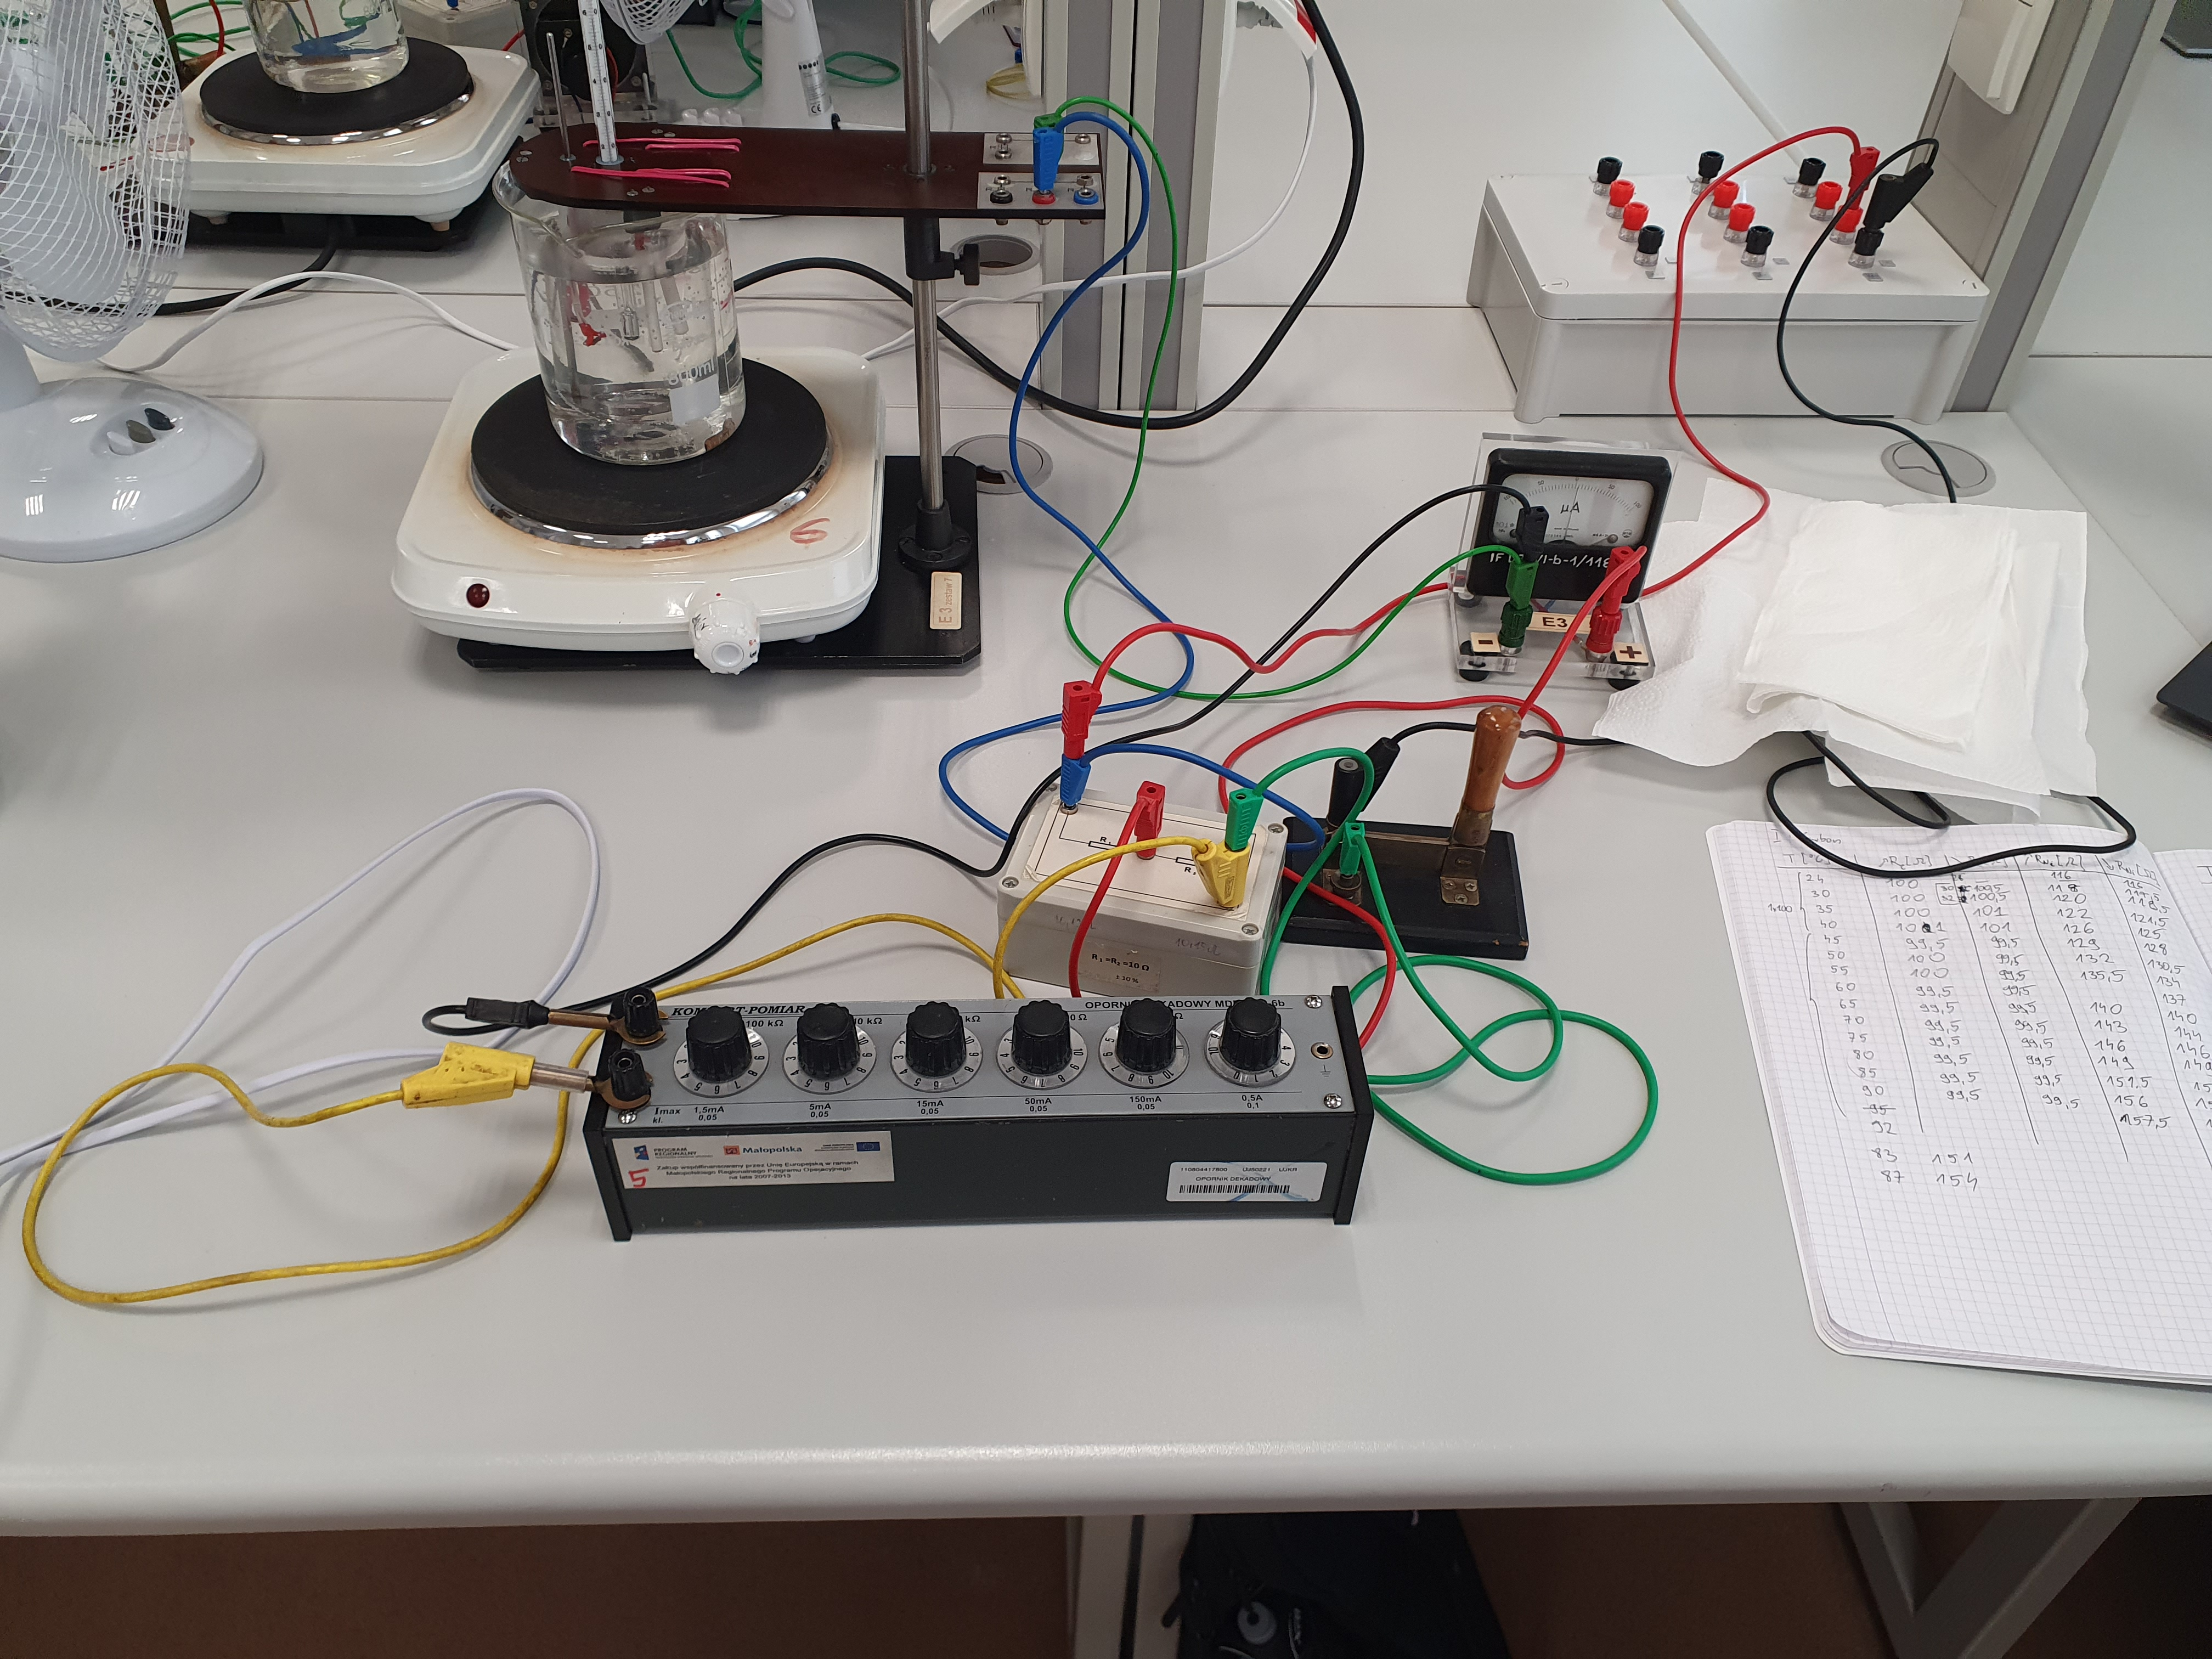
\includegraphics [width=0.95\columnwidth] {img/zdjecie-ukladu.jpg}
  \caption{\small Zdjęcie układu pomiarowego z widocznym stworzonym układem mostka Wheastone'a zawierającym: m.in opornicę dekadową, oporniki drutowe, źródło zasilania oraz klucz. Dodatkowo na zdjęciu widoczny jest termometr rtęciowy oraz aparatura do podgrzewania cieczy, w której znajdują się oporniki.}
  \label{fig:zdjecie-ukladu}
\end{figure}

\section{Przebieg pomiarów}
\subsection{Omomierz}
Do bezpośrednich pomiarów oporów użyty został multimetr \textit{Metex M-4650CR}.
W funkcji omomierza jego niepewności graniczne dla zakresu odpowiednio 
$200~\Omega$ ($\Delta R_{\mathrm{O}, 200}$) oraz 
$2~\kOhm$ ($\Delta R_{\mathrm{O}, 2\mathrm{k}}$) są funkcjami zmierzonej wartości, co przedstawiają zależności~(\ref{eq:omomierz-niepewnosci})~\cite{metex-instrukcja}.
\begin{equation}
\begin{split}
    \Delta R_{\mathrm{O}, 200} 
        &= 0.2\% \cdot R_{\mathrm{X}} + 0.05~\Omega \\
    \Delta R_{\mathrm{O}, 2\mathrm{k}}
        &= 0.15\% \cdot R_{\mathrm{X}} + 0.3~\Omega
    \label{eq:omomierz-niepewnosci}
\end{split}
\end{equation}

\subsection{Opornica dekadowa}
Do ustawiania zmiennej rezystancji użyta została opornica dekadowa \textit{MDR-93/2-6b} marki \textit{Kompakt-Pomiar}. Najmniejsza dekada pozwala na zmianę oporu o $\pm 1\Omega$.
Niepewność graniczna ustawionego oporu $R_{\mathrm{OD}}$ jest funkcją ustawionego oporu na najmniejszej dekadzie ($R_{1\Omega}$) oraz oporu ustawionego na pozostałych dekadach ($R_{\ge10\Omega}$), co przedstawia zależność~(\ref{eq:opornik-dekadowy-niepewnosci})~\cite{mdr93-instrukcja}. Jako niepewność rezystancji zerowej została wzięta wartość nieco większa, niż w cytowanej instrukcji, gdyż użyty opornik ma o jedną dekadę więcej.
\begin{equation}
    \Delta R_{\mathrm{OD}} 
        = 0.05\% \cdot R_{\ge10\Omega}
            + 0.1\% \cdot R_{1\Omega}
            + 0.01~\Omega
    \label{eq:opornik-dekadowy-niepewnosci}
\end{equation}

Błąd ustawienia oporu wyrażony zależnością~(\ref{eq:opornik-dekadowy-niepewnosci}) jest jednak bardzo mały (rzędu $10~\mathrm{m\Omega}$), w porównaniu z wartością, o jaką jesteśmy w stanie modyfikować uzyskany opór.
Za realna niepewność graniczną pomiaru oporu przy użyciu opornicy dekadowej przyjmiemy więc wartość najmniejszej dekady, a więc: $\Delta R_{\mathrm{D}} = 1~\Omega$.

\section{Wyniki i dyskusja}
\subsection{Oporniki w temperaturze pokojowej}
Opór każdego z trzech oporników został zmierzony dwiema metodami: przy użyciu omomierza oraz za pomocą opornicy dekadowej. Wyniki przedstawia Tabela~\ref{tab:oporniki-opor}.

\begin{table}[ht]
\begin{center}
\renewcommand*{\tablename}{Tabela}
\caption{\small
Wyniki pomiarów oporników przy pomocy Omomierza $\RO$ (kolumna 2) oraz mostka Wheastone’a $\RM$ (kolumna 3) wraz z niepewnością graniczną pomiarów.
\vspace{0.15cm}
    \label{tab:oporniki-opor}}
    {\small
    \begin{tabular}{c r c}
    \hline \vspace{-0.35cm} \\
      Opornik & $\RO~[\Omega]$ 
      & $\RM~[\Omega]$ \\
      \hline \vspace{-0.2cm} \\
      C  &  99.95(25) & 101(1) \\
      Ni & 112.57(28) & 114(1) \\
      Pt & 108.75(27) & 109(1) \\
    \hline
    \end{tabular}}
    \end{center}
\end{table}

Jak widać w Tabeli~\ref{tab:oporniki-opor}, dla oporników węglowego oraz platynowego, różnica wyników pomiarów oboma metodami jest poniżej sumarycznego błędu granicznego ${(\Delta \RO +\Delta \RM)}$. Jedynie dla opornika niklowego, błąd wynosi około ${116\%~(\Delta \RO +\Delta \RM)}$.

\subsection{Oporniki połączone szeregowo}
Dla każdej z trzech różnych par oporników został stworzony układ dwóch oporników połączonych szeregowo. Dla każdego układu został zmierzony opór zastępczy dwiema metodami: przy użyciu omomierza oraz za pomocą opornicy dekadowej. Dodatkowo został policzony teoretyczny opór zastępczy przy użyciu zależności~(\ref{eq:oporniki-szeregowo-teoria}) oraz danych z Tabeli~\ref{tab:oporniki-opor}. Wyniki przedstawia Tabela~\ref{tab:oporniki-szeregowo-opor}.

\begin{table}[ht]
\begin{center}
\renewcommand*{\tablename}{Tabela}
\caption{\small
Wyniki pomiarów oporu par oporników ustawionych szeregowo przy pomocy omomierza $\RO$ (kolumna 2) oraz mostka Wheastone’a $\RM$ (kolumna 4).
Dodatkowo obliczone wartości teoretyczne z równania~(\ref{eq:oporniki-szeregowo-teoria}) dla pomiarów omomierzem $\ROT$ (kolumna 3) oraz mostka Wheastone’a $\RMT$ (kolumna 4).
\vspace{0.15cm}
    \label{tab:oporniki-szeregowo-opor}}
    {\small
    \begin{tabular}{c c c c c}
    \hline \vspace{-0.35cm} \\
      Opor. & $\RO[\Omega]$
      & $\ROT[\Omega]$
      & $\RM[\Omega]$
      & $\RMT[\Omega]$ \\
      \hline \vspace{-0.2cm} \\
      C,  Ni & 212.50(62) & 212.47(53) & 214(1) & 215(2) \\
      C,  Pt & 208.90(62) & 208.70(52) & 210(1) & 210(2) \\
      Ni, Pt & 221.50(64) & 221.27(55) & 223(1) & 223(2) \\
    \hline
    \end{tabular}}
    \end{center}
\end{table}

Jak widać w Tabeli~\ref{tab:oporniki-szeregowo-opor}, dla par węgiel+nikiel oraz węgiel+platyna, różnica wyników pomiarów dla każdej z czterech metod jest parami poniżej sumarycznego błędu granicznego ${(\Delta R_1 + \Delta R_2)}$.
Jedynie dla pary nikiel+platyna, różnica między wartością teoretyczną uzyskaną z pomiarów omomierzem $\ROT$ oraz bezpośredni pomiar mostkiem $\RM$ wynosi około ${113\%~(\Delta \ROT+\Delta \RM)}$.

\subsection{Oporniki połączone równolegle}
Dla każdej z trzech różnych par oporników został stworzony układ dwóch oporników połączonych równolegle. Został także stworzony układ wszystkich trzech oporników połączonych równolegle. Dla każdego układu został zmierzony opór zastępczy dwiema metodami: przy użyciu omomierza oraz za pomocą opornicy dekadowej. Dodatkowo został policzony teoretyczny opór zastępczy przy użyciu zależności~(\ref{eq:oporniki-rownolegle-teoria}) oraz danych z Tabeli~\ref{tab:oporniki-opor}. Wyniki przedstawia Tabela~\ref{tab:oporniki-rownolegle-opor}.

\begin{table}[ht]
\begin{center}
\renewcommand*{\tablename}{Tabela}
\caption{\small
Wyniki pomiarów oporu par oraz całej trójki oporników (ostatni rząd) ustawionych równolegle przy pomocy omomierza $\RO$ (kolumna 2) oraz mostka Wheastone’a $\RM$ (kolumna 4).
Dodatkowo obliczone wartości teoretyczne z równania~(\ref{eq:oporniki-rownolegle-teoria}) dla pomiarów omomierzem $\ROT$ (kolumna 3) oraz mostka Wheastone’a $\RMT$ (kolumna 4).
\vspace{0.15cm}
    \label{tab:oporniki-rownolegle-opor}}
    {\small
    \begin{tabular}{c c c c c}
    \hline \vspace{-0.35cm} \\
      Opor. & $\RO[\Omega]$
      & $\ROT[\Omega]$
      & $\RM[\Omega]$
      & $\RMT[\Omega]$ \\
      \hline \vspace{-0.2cm} \\
      C,  Ni & 52.98(16) & 52.932(93) & 53(1)    & 53.55(36) \\
      C,  Pt & 52.08(16) & 52.082(92) & 52.5(10) & 52.42(36) \\
      Ni, Pt & 55.31(17) & 55.301(96) & 56(1)    & 55.72(36) \\
      Trzy   & 35.63(13) & 35.603(51) & 36(1)    & 35.91(20) \\
    \hline
    \end{tabular}}
    \end{center}
\end{table}

Jak widać w Tabeli~\ref{tab:oporniki-rownolegle-opor}, dla par węgiel+platyna oraz nikiel+platyna, różnica wyników pomiarów dla każdej z czterech metod jest parami poniżej sumarycznego błędu granicznego $(\Delta R_1 + \Delta R_2)$.

Dla pary węgiel+nikiel różnica między wartością teoretyczną uzyskaną z pomiarów mostkiem $\RMT$ jest różna od wartości uzyskanych omomierzem 
o około ${112\%~(\Delta \RO + \Delta \RMT)}$ dla $\RO$
oraz o około ${138\%~(\Delta \ROT + \Delta \RMT)}$ dla $\ROT$.

Dla trójki oporników obie wartości teoretyczne $\ROT$ i $\RMT$ różnią się
o około ${125\%~(\Delta \ROT + \Delta \RMT)}$.

\subsection{Temperaturowa zależność oporu opornika węglowego}
Wszystkie pomiary oporu opornika węglowego dla różnych temperatur zamieszczone są w Tabeli~\ref{tab:opornik-weglowy-pomiary}. Umieszczona została tam też obliczona wartość średnia dla konkretnych temperatur.

\begin{table}[ht]
\begin{center}
\renewcommand*{\tablename}{Tabela}
\caption{\small
Wyniki pomiarów oporu opornika węglowego dla różnych temperatur podczas podgrzewania $R_{\mathrm{C \nearrow}}$ (kolumna 2), chłodzenia $R_{\mathrm{C \searrow}}$ (kolumna 3) oraz uzyskana wartość średnia $\bar{\RC}$ (kolumna 4).
\vspace{0.15cm}
    \label{tab:opornik-weglowy-pomiary}}
    {\small
    \begin{tabular}{c c c c c}
    \hline \vspace{-0.35cm} \\
      $T$ [$^{\circ}$C] & $R_{\mathrm{C\nearrow}}$ [$\Omega$] & $R_{\mathrm{C\searrow}}$ [$\Omega$] & $\bar{\RC}$ [$\Omega$] \\
      \hline \vspace{-0.2cm} \\
        24 & 100  & --    & 100    \\
        30 & 100  & 100.5 & 100.25 \\
        32 & --   & 100.5 & 100.5  \\
        35 & 100  & 101   & 100.5  \\
        40 & 101  & 101   & 101    \\
        45 & 99.5 & 99.5  & 99.5   \\
        50 & 100  & 99.5  & 99.75  \\
        55 & 100  & 99.5  & 99.75  \\
        60 & 99.5 & 99.5  & 99.5   \\
        65 & 99.5 & 99.5  & 99.5   \\
        70 & 99.5 & 99.5  & 99.5   \\
        75 & 99.5 & 99.5  & 99.5   \\
        80 & 99.5 & 99.5  & 99.5   \\
        85 & 99.5 & 99.5  & 99.5   \\
        90 & 99.5 & 99.5  & 99.5   \\
    \hline
    \end{tabular}}
    \end{center}
\end{table}

Pobieżna analiza danych z Tabeli~\ref{tab:opornik-weglowy-pomiary} pozwala ocenić, że nie udało się zmierzyć zmiany oporu przy zmianie temperatur dla opornika węglowego. Niemniej jednak obliczone wartości średnie z tabeli zostały użyte do dopasowania prostej przy pomocy regresji liniowej. Uzyskana została prosta o parametrach~(\ref{eq:regresja-wegiel-parametry}). Niepewności parametrów są niepewnościami standardowymi.
\begin{equation}
\begin{split}
    a &= -1.65(45) \cdot 10^{-2}~\mathrm{\frac{\Omega}{K}} \\
    b &= (105.3 \pm 1.5)~\Omega
    \label{eq:regresja-wegiel-parametry}
\end{split}
\end{equation}

Miara dopasowania $R^2$ ma wartość: $R^2 \approx 0.52$, co jest znacznie poniżej warunku dobrego dopasowania krzywej w regresji $R^2 \geq 0.99$ \cite{epa-8000d}.

Zmierzone wartości z Tabeli~\ref{tab:opornik-weglowy-pomiary} wraz z dopasowaną prostą o parametrach~(\ref{eq:regresja-wegiel-parametry}) zostały przedstawione na wykresie: Rysunek~\ref{img:opornik-weglowy-wykres}.
\begin{figure}[ht]
\centering
    
\begin{tikzpicture}
\begin{axis}[
    title={Opornik węglowy, a temperatura},
    xlabel={Temperatura $T$ [$^{\circ}$C]},
    ylabel={Opór $R$ [$\Omega$]},
    legend pos=north east,
    grid=both,
    minor tick num=1,
    % Tells pgfplots to skip over 'nan' entries safely
    unbounded coords=jump, 
    % Adjusts axis limits slightly so error bars aren't cut off
    enlarge x limits=0.05, 
    enlarge y limits=0.1,
]

\def\slope{-0.01649}
\def\intercept{100.76925}
        
\addplot [red, thick, domain=24:90, forget plot] {\slope*x + \intercept};

% Cooling Data (↘ R_c) - Empty Symbols
\addplot [
    only marks,
    mark=*,
    color=black,
    forget plot,
    mark options={fill=white},
    error bars/.cd,
        x dir=both, x fixed=1,
        y dir=both, y fixed=1,
] table [x=T, y=R_down] {
    T     R_up    R_down
    24    100     nan
    30    100     100.5
    32    nan     100.5
    35    100     101
    40    101     101
    45    99.5    99.5
    50    100     99.5
    55    100     99.5
    60    99.5    99.5
    65    99.5    99.5
    70    99.5    99.5
    75    99.5    99.5
    80    99.5    99.5
    85    99.5    99.5
    90    99.5    99.5
};

% Heating Data (↗ R_c) - Filled Symbols
\addplot [
    only marks,
    mark=*,
    color=black,
    forget plot,
    error bars/.cd,
        x dir=both, x fixed=1,
        y dir=both, y fixed=1,
] table [x=T, y=R_up] {
    T     R_up    R_down
    24    100     nan
    30    100     100.5
    32    nan     100.5
    35    100     101
    40    101     101
    45    99.5    99.5
    50    100     99.5
    55    100     99.5
    60    99.5    99.5
    65    99.5    99.5
    70    99.5    99.5
    75    99.5    99.5
    80    99.5    99.5
    85    99.5    99.5
    90    99.5    99.5
};

\addlegendimage{only marks, mark=*, black, error bars/.cd, y dir=both, y explicit}
\addlegendentry{Podgrzewanie: $T \nearrow$}

\addlegendimage{only marks, mark=*, black, mark options={fill=white}, error bars/.cd, y dir=both, y explicit}
\addlegendentry{Chłodzenie: $T \searrow$}

\addlegendimage{no markers, red, thick}
\addlegendentry{Regresja liniowa}

\end{axis}
\end{tikzpicture}

\caption{
    Zmierzone opory opornika węglowego dla różnych temperatur wraz z niepewnościami pomiarowymi oraz prostą $R=aT+b$ doprasowaną przy pomocy regresji liniowej.
}
\label{img:opornik-weglowy-wykres}
\end{figure}


Zależność~(\ref{eq:teoria:alpha-od-prostej}) pozwala teraz na wyliczenie temperaturowego współczynnika oporności właściwej dla opornika węglowego $\alpha_{\mathrm{C}}$ przy pomocy współczynników prostej o wartościach~(\ref{eq:regresja-wegiel-parametry}). Uzyskana została wartość~(\ref{eq:wegiel-wspolczynnik}). Niepewność jest niepewnością standardową.
\begin{equation}
    \alpha_{\mathrm{C}} = -1.64(43) \cdot 10^{-4}~\frac{1}{ \mathrm{K} }
    \label{eq:wegiel-wspolczynnik}
\end{equation}

\subsection{Temperaturowa zależność oporu opornika niklowego}
Ze względu na trudności podczas eksperymentu, podgrzewanie odbyło się w dwóch osobnych seriach: Pierwsza dla temperatur ${75^\circ\mathrm{C} - 92^\circ\mathrm{C}}$, druga dla temperatur ${28^\circ\mathrm{C} - 70^\circ\mathrm{C}}$. Wszystkie pomiary oporu opornika niklowego dla różnych temperatur zamieszczone są w Tabeli~\ref{tab:opornik-niklowy-pomiary}. Umieszczona została tam też obliczona wartość średnia dla konkretnych temperatur.

\begin{table}[ht]
\begin{center}
\renewcommand*{\tablename}{Tabela}
\caption{\small
Wyniki pomiarów oporu opornika niklowego dla różnych temperatur podczas podgrzewania $R_{\mathrm{Ni \nearrow_1}}$ (kolumna 2), drugiego podgrzewania $R_{\mathrm{Ni \nearrow_2}}$ (kolumna 3), chłodzenia $R_{\mathrm{Ni \searrow}}$ (kolumna 4) oraz uzyskana wartość średnia $\bar{R}_{\mathrm{Ni}}$ (kolumna 5).
\vspace{0.15cm}
    \label{tab:opornik-niklowy-pomiary}}
    {\small
    \begin{tabular}{c l l l l}
    \hline \vspace{-0.35cm} \\
      $T$ [$^{\circ}$C] & $R_{\mathrm{Ni\nearrow_1}}$ [$\Omega$] & $R_{\mathrm{Ni\nearrow_2}}$ [$\Omega$] & $R_{\mathrm{Ni\searrow}}$ [$\Omega$] & $\bar{R}_{\mathrm{Ni}}$ [$\Omega$] \\
      \hline \vspace{-0.2cm} \\
        28 & --    & 116   & 116   & 116    \\
        30 & --    & 118   & 117.5 & 117.75 \\
        32 & --    & 120   & 119.5 & 119.75 \\
        35 & --    & 122   & 121.5 & 121.75 \\
        40 & --    & 126   & 125   & 125.5  \\
        45 & --    & 129   & 128   & 128.5  \\
        50 & --    & 132   & 130.5 & 131.25 \\
        55 & --    & 135.5 & 134   & 134.75 \\
        60 & --    & 138.5 & 137   & 137.75 \\
        65 & --    & 141   & 140   & 140.5  \\
        70 & --    & 144   & 144   & 144    \\
        75 & 146   & --    & 146   & 146    \\
        80 & 149   & --    & 149   & 149    \\
        85 & 151.5 & --    & 152   & 151.75 \\
        90 & 156   & --    & 154.5 & 155.25 \\
        92 & 157.5 & --    & 157.5 & 157.5  \\
    \hline
    \end{tabular}}
    \end{center}
\end{table}

Obliczone wartości średnie z Tabeli~\ref{tab:opornik-niklowy-pomiary} zostały użyte do dopasowania prostej przy pomocy regresji liniowej. Uzyskana została prosta o parametrach~(\ref{eq:regresja-nikiel-parametry}). Niepewności parametrów są niepewnościami standardowymi.
\begin{equation}
\begin{split}
    a &= 0.6203(81)~\mathrm{\frac{\Omega}{K}} \\
    b &= (-69.5 \pm 2.7)~\Omega
    \label{eq:regresja-nikiel-parametry}
\end{split}
\end{equation}

Miara dopasowania $R^2$ ma wartość: $R^2 = 0.99767$, co spełnia warunek dobrego dopasowania krzywej w regresji $R^2 \geq 0.99$ \cite{epa-8000d}.

Zmierzone wartości z Tabeli~\ref{tab:opornik-niklowy-pomiary} wraz z dopasowaną prostą o parametrach~(\ref{eq:regresja-nikiel-parametry}) zostały przedstawione na wykresie: Rysunek~\ref{img:opornik-nikolwy-wykres}.
\begin{figure}[ht]
\centering
    
\begin{tikzpicture}
\begin{axis}[
    title={Opornik niklowy, a temperatura},
    xlabel={Temperatura $T$ [$^{\circ}$C]},
    ylabel={Opór $R$ [$\Omega$]},
    legend pos=north west,
    grid=both,
    minor tick num=1,
    % Tells pgfplots to skip over 'nan' entries safely
    unbounded coords=jump, 
    % Adjusts axis limits slightly so error bars aren't cut off
    enlarge x limits=0.05, 
    enlarge y limits=0.1,
]

\def\slope{0.62028}
\def\intercept{99.9313}
        
\addplot [red, thick, domain=28:92, forget plot] {\slope*x + \intercept};

% Cooling Data (↘ R_c) - Empty Symbols
\addplot [
    only marks,
    mark=*,
    color=black,
    forget plot,
    mark options={fill=white},
    error bars/.cd,
        x dir=both, x fixed=1,
        y dir=both, y fixed=1,
] table [x=T, y=R_down] {
    T     R_up  R_down
    28	116	116
    30	118	117.5
    32	120	119.5
    35	122	121.5
    40	126	125
    45	129	128
    50	132	130.5
    55	135.5	134
    60	138.5	137
    65	141	140
    70	144	144
    75	146	146
    80	149	149
    85	151.5	152
    90	156	154.5
    92	157.5	157.5
};

% Heating Data (↗ R_c) - Filled Symbols
\addplot [
    only marks,
    mark=*,
    color=black,
    forget plot,
    error bars/.cd,
        x dir=both, x fixed=1,
        y dir=both, y fixed=1,
] table [x=T, y=R_up] {
    T     R_up  R_down
    28	116	116
    30	118	117.5
    32	120	119.5
    35	122	121.5
    40	126	125
    45	129	128
    50	132	130.5
    55	135.5	134
    60	138.5	137
    65	141	140
    70	144	144
    75	146	146
    80	149	149
    85	151.5	152
    90	156	154.5
    92	157.5	157.5
};

\addlegendimage{only marks, mark=*, black, error bars/.cd, y dir=both, y explicit}
\addlegendentry{Podgrzewanie: $T \nearrow$}

\addlegendimage{only marks, mark=*, black, mark options={fill=white}, error bars/.cd, y dir=both, y explicit}
\addlegendentry{Chłodzenie: $T \searrow$}

\addlegendimage{no markers, red, thick}
\addlegendentry{Regresja liniowa}

\end{axis}
\end{tikzpicture}

\caption{
    Zmierzone opory opornika niklowego dla różnych temperatur wraz z niepewnościami pomiarowymi oraz prostą $R=aT+b$ doprasowaną przy pomocy regresji liniowej.
}
\label{img:opornik-nikolwy-wykres}
\end{figure}


Zależność~(\ref{eq:teoria:alpha-od-prostej}) pozwala teraz na wyliczenie temperaturowego współczynnika oporności właściwej dla opornika niklowego $\alpha_{\mathrm{Ni}}$ przy pomocy współczynników prostej o wartościach~(\ref{eq:regresja-nikiel-parametry}). Uzyskana została wartość~(\ref{eq:nikiel-wspolczynnik}). Niepewność jest niepewnością standardową.
\begin{equation}
    \alpha_{\mathrm{Ni}} = 5.52(37) \cdot 10^{-3}~\frac{1}{ \mathrm{K} }
    \label{eq:nikiel-wspolczynnik}
\end{equation}

\section{Podsumowanie i wnioski}
\subsection{Dwie metody pomiarów oporu}
\label{sec:podsumowanie:dwie-metody-pomiarow}
W znacznej większości pomiary oporu obiema metodami dawały analogiczne wyniki mieszczące się w swoich niepewnościach granicznych. Dla kilku par pomiarów wystąpiła jednak sytuacja, że wyniki różniły się o $100\%-200\%$ sumy niepewności granicznych. Wystąpienie taki sytuacji sugeruje, że przyjęte niepewności są w rzeczywistości zbyt małe.

Dodatkowo podczas eksperymentu założony został zerowy opór przewodów. Taka idealizacja układu pomiarowego mogła doprowadzić do zignorowania czynników, które w sposób istotny wpływają na otrzymywany rezultat.

Bardzo istotną poszlaką jest fakt, że w \textbf{każdym} pomiarze odczyt oporu  mostka okazał się większy, niż odczyt omomierza. Jest to moim zdaniem jednoznacznym dowodem, że któryś z pomiarów obarczony jest stałym błędem systematycznym (odchyleniem w jedną stronę).

Dodatkowo przy ustalaniu niepewności pomiarów oporu mostkiem zignorowana została dokładność amperomierza, przy pomocy którego kalibrowano opornicę dekadową.

\subsection{Łączenie oporników szeregowo i równolegle}
Pomiary układów oporników dawały wyniki zgodne z przewidywaniami teoretycznymi, z zastrzeżeniem do drobnych odchyleń opisanych w podrozdziale~\ref{sec:podsumowanie:dwie-metody-pomiarow}. Udało się tym samym potwierdzić eksperymentalnie przewidywania teoretyczne.

\subsection{Temperaturowa zależność oporu opornika węglowego}
Wyznaczenie temperaturowej zależności oporu opornika węglowego zakończyło się niepowodzeniem. Dobitnie o fiasku przedsięwzięcia świadczy skrajnie niska miara dopasowania prostej: $R^2 \approx 0.52$.

Jako przyczynę niepowodzenia wskazałbym głównie fakt bardzo niewielkiej dokładność aparatury pomiarowej (rzędu $1\Omega$) w porównaniu z rejestrowanymi różnicami w oporze (maksymalnie $1.5\Omega$). Powoduje to, że błędy pomiaru są w praktyce większe, niż faktyczne różnice w oporze powodowane przez zmianę temperatury.

Dodatkowym świadectwem klęski jest niemonotoniczność odczytywanych wartości. Pomiary na samym początku delikatnie rosną (o ok. $1\Omega$) w temperaturach $20^{\circ}\mathrm{C}-40^{\circ}\mathrm{C}$, by następnie opaść (o ok. $1.5\Omega$) w temperaturach $40^{\circ}\mathrm{C}-60^{\circ}\mathrm{C}$, po czym przybierać dokładnie tę samą wartość aż do maksymalnej temperatury $90^{\circ}\mathrm{C}$. Przy takiej zależności zupełnie nie dziwi tak słaba miara dopasowania prostej $R^2$.

Koniec końców otrzymana wartość temperaturowego współczynnika oporności właściwej dla opornika węglowego $\alpha_{\mathrm{C}} = -1.64(43) \cdot 10^{-4}~\frac{1}{ \mathrm{K} }$ różni się od wartości tablicowej $\alpha_{\mathrm{C, T}} = -5 \cdot 10^{-4}~\frac{1}{ \mathrm{K} }$ \cite{pracownia-fizyczna-e3} o niemalże $8 \sigma_{ \alpha_{\mathrm{C}} }$!

\subsection{Temperaturowa zależność oporu opornika niklowego}
W przypadku pomiaru oporu opornika niklowego w trakcie podgrzewania nie udało się niestety uzyskać jednej serii dla całego przedziału temperatur. Tym niemniej uzyskane dwie serie wydają się być nieobarczone różnymi błędami statystycznymi (brak przeskoku w momencie przejścia) oraz spójne z wartościami uzyskanymi podczas całościowej serii chłodzenia.

Wyznaczenie temperaturowej zależności oporu opornika niklowego okazała się znacznie większym sukcesem niż w wypadku węglowego. Dane pomiarowe są monotoniczne, a umieszczone na wykresie przypominają linię prostą. W sposób obiektywny świadczy o tym wysoka miara dopasowania prostej: $R^2 = 0.99767$.

Otrzymana wartość temperaturowego współczynnika oporności właściwej dla opornika niklowego $\alpha_{\mathrm{Ni}} = 5.52(37) \cdot 10^{-3}~\frac{1}{ \mathrm{K} }$ różni się od wartości tablicowej $\alpha_{\mathrm{Ni, T}} = 6 \cdot 10^{-3}~\frac{1}{ \mathrm{K} }$ \cite{pracownia-fizyczna-e3} o około $1.3 \sigma_{ \alpha_{\mathrm{Ni}} }$, co jest wartością w pełni zadowalającą.

\section{Podziękowania}
Dziękuję Panu dr dr Pawłowi Nicie za cenne dyskusje i opiekę podczas przeprowadzenia eksperymentu.

\begin{thebibliography}{7}
    \bibitem{epa-8000d} US Environmental Protection Agency (EPA), \emph{Method 8000D: Determinative Chromatographic Separations}, (\url{https://www.epa.gov/sites/default/files/2015-12/documents/8000d.pdf}) (dostęp:~21.03.2026).

    \bibitem{metex-instrukcja} Zakład Fizyki, \emph{Instrukcja obsługi multimetrów cyfrowych Metex}, Politechnika Łódzka (\url{https://fizyka.p.lodz.pl/pl/download/resource/1295/}) (dostęp:~28.03.2026).

    \bibitem{mdr93-instrukcja} INCO/KOMPART-POMIAR, \emph{Opornik dekadowy MDR-93. Instrukcja obsługi / DTR}, (\url{https://metrologia-elektryczna.po.edu.pl/wp-content/uploads/2024/05/Opornik-dekadowy-MDR-93.pdf}) (dostęp:~28.03.2026).
    
    \bibitem{pracownia-fizyczna-e3} I~Pracownia Fizyczna, \emph{Temperaturowa zależność oporu przewodników (E3)}, Instytut Fizyki~UJ (\url{https://1pf.if.uj.edu.pl/materialy-do-cwiczen/spis-cwiczen}) (dostęp:~28.03.2026).
\end{thebibliography}


\end{document}